\section{Key network parameters and derived cost functions}
\label{ch1:sec:key-network-parameters}

Two distinct approaches have emerged to quantitatively improve the performance of a system: either ``cost'' is reduced or ``utility'' is maximised.
Both approaches rely on a mathematical explanation of underlying features that relate to performance of the system.
The choice for this piece of work was to associate a cost to each key network parameter, for the reason that cost functions can be minimised towards a finite value, i.e. zero.
Utility maximisation on the other hand is a theoretically unbound problem that can only reach a maximum, if its maximum can be estimated in advance.
In other words, solutions to a cost function where the resulting cost is zero, are by definition part of the set of optimal solutions.
Determining the set of optimal solutions for the maximisation of a utility function is however more difficult.

\nomenclature[I]{$t$}{Time-steps of the simulation, where $t \in \{1,\Delta t, 2\Delta t,\dots,T\}$ (Chapter \ref{ch1})}
\nomenclature[I]{$\Delta t$}{Sample time, where $\Delta t \in \mathbb{Z}_{\geq0}$ (Chapter \ref{ch1})}
\nomenclature[I]{$T$}{Length of simulation, where $T \in \mathbb{Z}_{\geq0}$ (Chapter \ref{ch1})}

With this in mind, the key network parameters are defined and their corresponding cost functions are introduced.
In this piece of work, power flow simulations are run at discrete times, $t$, which are separated by a sampling period $\Delta t$. 
The model used for these simulations is the IEEE LV Test Case, which consists of 906 three phase buses, resulting in a total of 2718 nodes.
For each node, complex currents and voltages can be obtained, making the number of parameters to chose from nearly inexhaustible.
In reality however, a power distribution network can only be observed at a limited number of measuring points.
For the NTVV project, these points were at the substation and the ESMU's Point of Common Coupling (PCC).
Therefore, all derived network parameters that could be obtained in reality are seen as ``realistic parameters'', despite the fact that all key network parameters are extracted from power flow simulations.
The remaining key network parameters, i.e. those that could not easily be obtained in reality, are therefore referred to as ``theoretical parameters''.

Due to the high number of these theoretical parameters, only a subset of them is used.
The choice of parameters is based on their importance, role and impact on the actual network operation.
A list of all key network parameters is presented below, and in this list all theoretical key network parameters are marked with a dagger ($\dagger$).

\begin{itemize}
	\item Voltages at substation transformer's secondary winding
	\item Voltages at ESMU's PCC
	\item Voltages at customer lateral$^{\dagger}$
	\item Total power flow
	\item Substation line utilisation
	\item Maximum line utilisation$^{\dagger}$
	\item Distribution losses$^{\dagger}$
\end{itemize}


The following three substations cover all key network parameters, by detailing the cost functions relating to: voltages, powers and currents.

\subsection{Voltage related cost functions}
\label{ch1:subsec:voltages-related-cost-functions}

\nomenclature[I]{$v_{\text{ss},\phi}$}{Phase voltage at substation for phase $\phi$ at time $t$, where $\textbf{v}_{ss}(t) = (v_{\text{ss},\phi}(t))$ (Chapter \ref{ch1})}
\nomenclature[I]{$\textbf{v}_{ss}(t)$}{Phase voltage vector at time $t$, where $\textbf{v}_\text{ss}(t) \in \mathbb{R}^{\Phi}$ (Chapter \ref{ch1})}
\nomenclature[I]{$\phi$}{Phase number, where $\phi \in \{1, \dots, \Phi\}$ (Chapter \ref{ch1})}
\nomenclature[I]{$\Phi$}{Number of phases, where $\Phi \in \mathbb{Z}_{>0}$ here $\Phi = 3$ (Chapter \ref{ch1})}
\nomenclature[I]{$\zeta_\text{voltage}(\textbf{v}(t))$}{Voltage deviation cost for voltage vector $\textbf{v}$ at time $t$, where $\zeta_\text{voltage}(\textbf{v}(t)) \in \mathbb{R}_{\geq0}$ (Chapter \ref{ch1})}
\nomenclature[I]{$V_\text{ss}$}{Nominal substation voltage, where $V_\text{ss} \in \mathbb{R}$ (Chapter \ref{ch1})}
\nomenclature[I]{$V_h$}{High-voltage threshold of statutory voltage band, where $V_h \in \mathbb{R}$ (Chapter \ref{ch1})}
\nomenclature[I]{$V_l$}{Low-voltage threshold of statutory voltage band, where $V_l \in \mathbb{R}$ (Chapter \ref{ch1})}

In the UK, LV networks operate at a nominal voltage of 230V Phase-to-Neutral (P2N) or 400V Phase-to-Phase (P2P).
Substations supply electricity to a three-phase cable, i.e. the feeder, and  link to MV distribution networks, which operate at 11kV P2P.
In an ideal case the voltage measured at the substation transformer's secondary winding remains constant as load changes.
But in reality, internal losses (e.g. conductive losses and magnetic leakage) lead to a dropping voltage level, when load increases.
Therefore, any deviation from the substation's nominal voltage can be seen as an indication of suboptimal network operation.

The ``voltage deviation cost function'' $\zeta_\text{voltage}(\textbf{v}(t))$ captures this suboptimal operation.
This cost function is defined for a multi-phase complex voltage vector as $\textbf{v}(t)$ where $\textbf{v}(t) = (v_\phi(t))$, where $\phi$ is the phase number and where $t$ the time at which the measurement was taken.
Both phase and time are discrete, i.e. $\phi \in \{1,\dots,\Phi\}$ where $\Phi \in \mathbb{Z}_{>0}$ and $t \in \mathbb{Z}_{\geq0}$.
When using the three-phase substation voltage vector, $\textbf{v}_{ss}(t)$ (where $\textbf{v}_{ss}(t) = (v_{\text{ss},\phi}(t))$), with this cost function, any drop in transformer voltage results in a positive cost.

\begin{equation}
\begin{split}
	\zeta_\text{voltage}(\textbf{v}(t)) :=& \sum_{\phi=1}^{\Phi}{\begin{cases}
		\zeta_h(v_{\phi}(t)) & \text{if } V_{ss} \leq v_\phi\\
		\zeta_l(v_{\phi}(t)) & \text{otherwise}\\
	\end{cases}} \forall t\\
	&\text{ where } \Phi \in \mathbb{Z}^{>0}
\end{split}
\label{ch1:equ:voltage-deviation}
\end{equation}

In this voltage cost function, $\Phi$ represents the number of phases (i.e. $\Phi = 3$), and $\zeta_h(v)$ and $\zeta_l(v)$ are two functions that convert a single voltage value, i.e. $v_p$, into a normalised positive cost based upon the direction of voltage deviation.
E.g. if the voltage $v_p$ is greater than or equal to the nominal substation voltage, $V_{ss}$, then the result from $\zeta_h(v)$ is used as a cost; otherwise the result from $\zeta_l(v)$ is used.
In order to define these two functions, the corresponding high and low voltage thresholds, respectively $V_h$ and $V_l$, are introduced.
With those high and low voltage bands, $V_{ss}$ has to be chosen in order to satisfy the following inequality:

\begin{equation}
	V_l < V_{ss} < V_h
\end{equation}

For the presented work, these two voltage thresholds are based on the UK's nominal LV voltage range of +10\% -6\% around $V_n$, i.e. 230V P2N.

\begin{equation}
	\zeta_h(v) := \alpha \left|\frac{v-V_{ss}}{V_h-V_{ss}}\right|^{\beta}
	\label{ch1:equ:high-voltage-threshold-cost-complete}
\end{equation}

\begin{equation}
	\zeta_l(v) := \alpha \left|\frac{V_{ss}-v}{V_{ss}-V_l}\right|^{\beta}
	\label{ch1:equ:low-voltage-threshold-cost-complete}
\end{equation}

In this context of defining $\zeta_{voltage}$, the variable $\alpha$ is used as the functions' linear weight that scales the corresponding cost, and the variable $\beta$ linearly increases the functions' gradients as voltage continues to deviate.
More specifically, $\alpha$ determines the value of the functions at voltages $V_l$ and $V_h$, where $\alpha \in \mathbb{R}^{>0}$; for example, when $\alpha = 1$, then $\zeta_{h}(v_l) = 1$.
$\beta$ on the other hand may take any value in the range of $\mathbb{R}^{>2}$, to assure a continuously differentiable cost function.
Both $\alpha$ and $\beta$ were treated as constants and, for the scope of this work, set to $1$ and $2$, respectively.
Substituting these values into Equations \ref{ch1:equ:high-voltage-threshold-cost-complete} and \ref{ch1:equ:low-voltage-threshold-cost-complete}, simplifies the high and low cost functions to:

\begin{equation}
	\zeta_h(v) := \left|\frac{v-V_{ss}}{V_h-V_{ss}}\right|^{2}
	\label{ch1:equ:high-voltage-threshold-cost-simple}
\end{equation}

\begin{equation}
	\zeta_l(v) := \left|\frac{V_{ss}-v}{V_{ss}-V_l}\right|^{2}
	\label{ch1:equ:low-voltage-threshold-cost-simple}
\end{equation}


In this voltage cost function, $\Phi$ represents the number of phases (i.e. $\Phi = 3$), and $\zeta_h(v_\phi)$ and $\zeta_l(v_\phi)$ are two functions that convert a single voltage value, i.e. $v_\phi$, into a normalised positive cost based upon the direction of voltage deviation.
High and low voltage thresholds, respectively $V_h$ and $V_l$, are introduced in order to define these two functions.
When choosing these two thresholds, then they must also satisfy the following inequality:

\begin{equation}
	V_l < V_\text{ss} < V_h
\end{equation}


For the work presented here, these two thresholds are based on the UK's nominal LV voltage range of +10\% -6\% around $V_n$, i.e. 230V P2N.
As a result, the following upper and lower threshold functions are defined, in order to form a continuously differentiable cost function with a single zero tangent.

\begin{equation}
	\zeta_h(v_\phi) := \left(\frac{v_\phi-V_\text{ss}}{V_h-V_\text{ss}}\right)^{2}
	\label{ch1:equ:high-voltage-threshold-cost-simple}
\end{equation}

\begin{equation}
	\zeta_l(v_\phi) := \left(\frac{V_\text{ss}-v_\phi}{V_\text{ss}-V_l}\right)^{2}
	\label{ch1:equ:low-voltage-threshold-cost-simple}
\end{equation}

Substations may raise the voltage above the nominal LV voltage level, since voltage levels drop continuously along a purely consumptive feeder.
The impact on the cost function $\zeta_\text{voltage}(\textbf{v})$ when $V_\text{ss}$ is increased is shown in Figure \ref{ch1:fig:voltage-deviation} (for simplicity a single-phase voltage vector is shown, i.e. $\Phi = 1$).

\begin{figure}\centering
	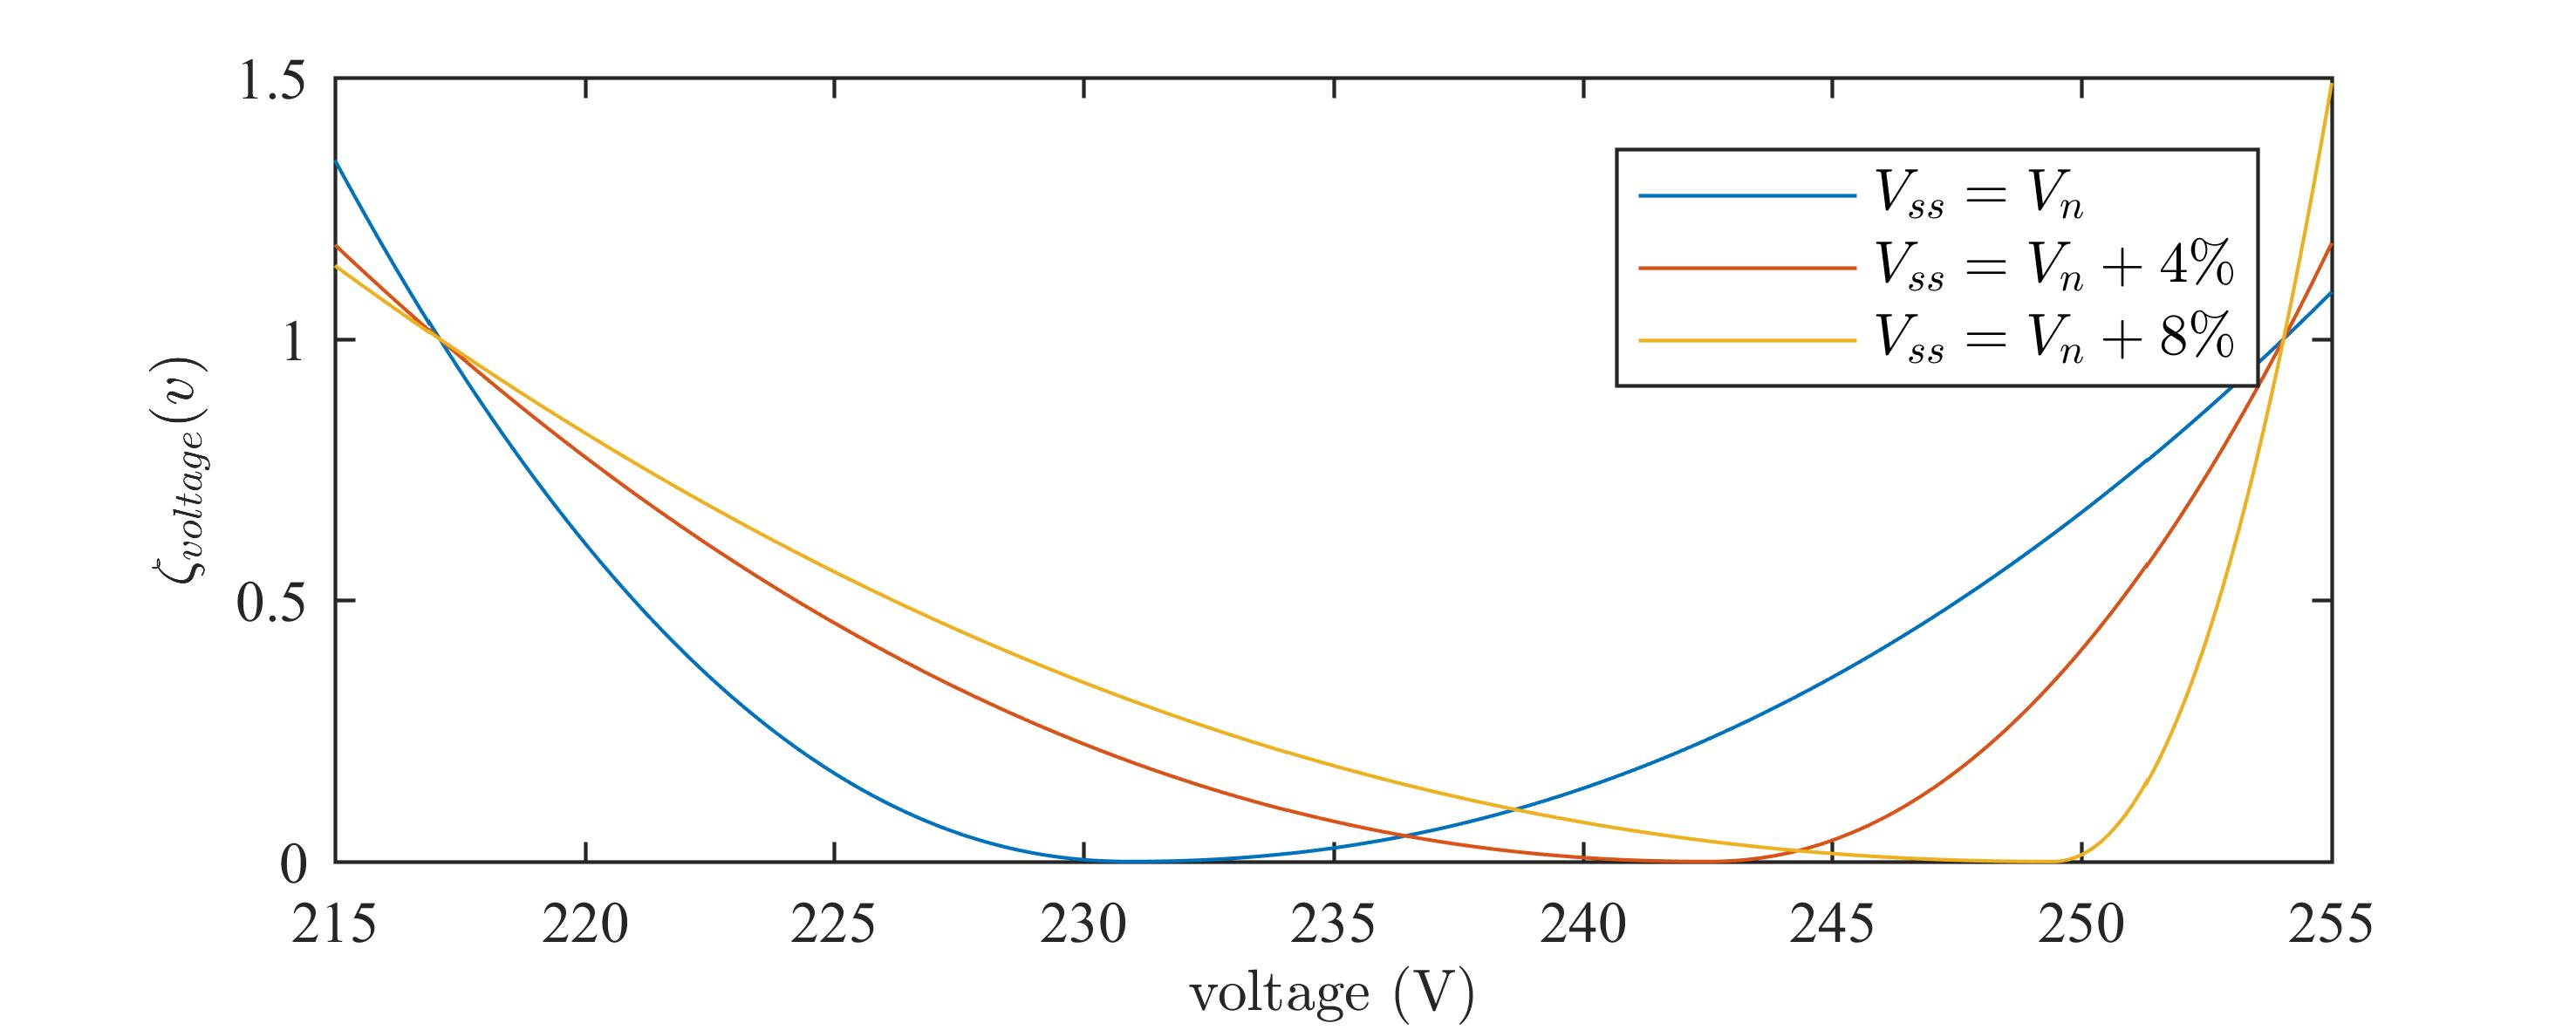
\includegraphics{_chapter1/fig/voltage-deviation}
	\caption{Cost function $\zeta_\text{voltage}(v_\phi)$ values for different substation voltages}	
	\label{ch1:fig:voltage-deviation}
\end{figure}

In this figure, it can be seen that $\zeta_\text{voltage}(\textbf{v})$ at the thresholds $V_l$ and $V_h$ equates to one, and to zero at the set substation voltage, even when this voltage is risen.
This intentional feature is demonstrated by raising $V_\text{ss}$ from $V_n$ by +4\% and +8\%.
At the ESMU's Point of Common Coupling (PCC), the device has access to all three phases of the feeder.
One can assume that the line voltage along a purely consumptive feeder will drop continuously.
Reasons behind this voltage drop are the resistive and inductive losses in the distribution lines, which are amplified with proximity to the substation, due to aggregated load currents form ``down stream'' customers.
Under heavy load conditions, this voltage is likely drop below the statutory operation limit.
Since this limit is an operational constraint for DNOs, it must not be violated.

To mitigate this voltage drop, power is injected into the feeder at the ESMU's PCC.
Doing so increases the voltage at its PCC and surrounding nodes, since the portion of load current that would normally be supplied by the substation is now delivered by the ESMU.
This effect when injecting power is sketched in the Figure \ref{ch1:fig:sketch-voltage-esmu} below.

\begin{figure}\centering
	\subfloat[Voltage drop along feeder without ESMU intervention]{%
		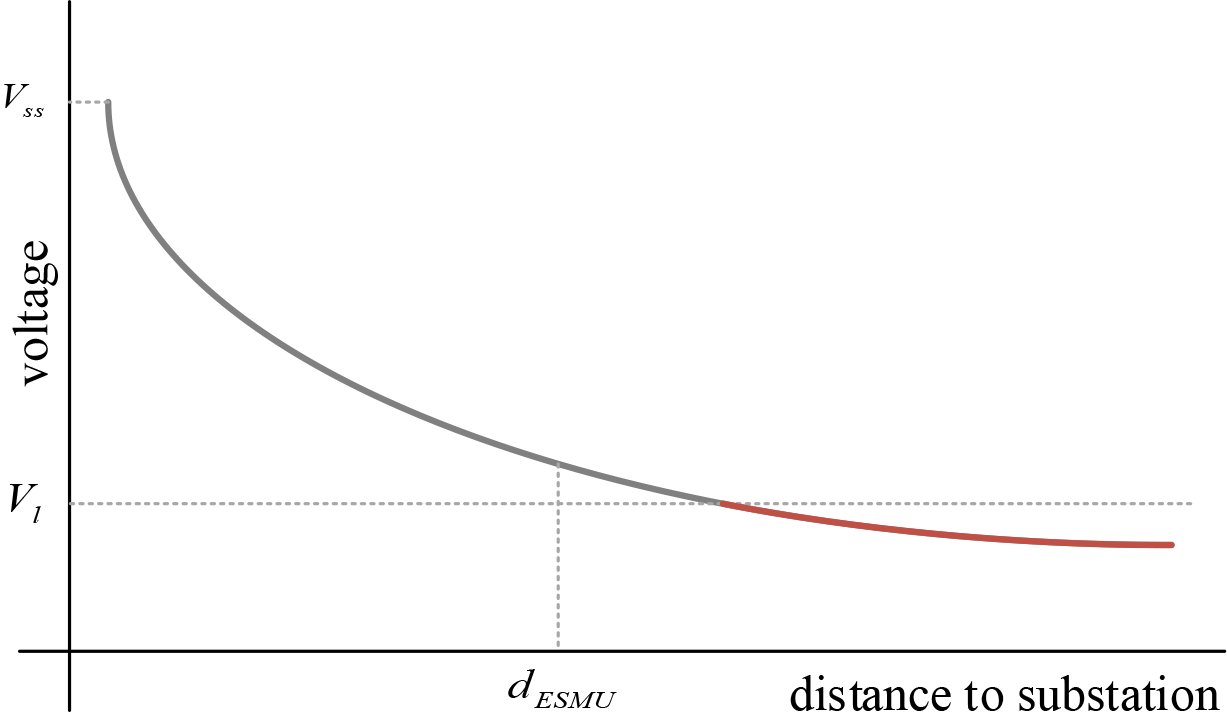
\includegraphics[width=0.45\textwidth]{_chapter1/fig/sketch-voltage-esmu-normal}%
		\label{ch1:subfig:sketch-voltage-esmu-normal}%
		}
	\hspace{5mm}
	\subfloat[Voltage drop along feeder with ESMU intervention]{%
		
\includegraphics[width=0.45\textwidth]{_chapter1/fig/sketch-voltage-esmu-boost}%
		\label{ch1:subfig:sketch-voltage-esmu-boost}%
		}
	\caption{Benefits of ESMU power injection on the voltage drop along the feeder}
	\label{ch1:fig:sketch-voltage-esmu}
\end{figure}

\nomenclature[I]{$v_{\text{ESMU},\phi}(t)$}{Phase voltage at ESMU for phase $\phi$ at time $t$, where $\textbf{v}_{ESMU}(t) = (v_{\text{ESMU},\phi}(t))$ and $v_{\text{ESMU},\phi}(t) \in \mathbb{C}$ (Chapter \ref{ch1})}
\nomenclature[I]{$\textbf{v}_\text{ESMU}(t)$}{Multi-phase voltage vector at ESMU at time $t$, where $\textbf{v}_{ESMU}(t) = (v_{\text{ESMU},\phi}(t))$ and $v_{\text{ESMU},\phi}(t) \in \mathbb{C}^{\Phi}$ (Chapter \ref{ch1})}

In this figure, the expected voltage drop along the entire feeder is sketched. 
It can be seen how the voltage of the feeder's tailing section can potentially drop below $V_l$, but ESMU's intervention can alleviate some load and bring voltages back within operational bounds.
The three-phase ESMU voltage, $\textbf{v}_{ESMU}(t)$ (where $\textbf{v}_{ESMU}(t) = (v_{\text{ESMU},\phi}(t))$) is seen as a realistic key network parameter, which is also used in combination with a cost function.
In fact, $\textbf{v}_{ESMU}(t)$ is used with cost function, $\zeta_\text{voltage}(\textbf{v}(t))$, which was defined in Equation \ref{ch1:equ:voltage-deviation}.
This is the same cost function (i.e. $\zeta_\text{voltage}(\textbf{v})$) that was used to asses the deviation in transformer voltage.
Therefore, the resulting cost can be formulated as $\zeta_\text{voltage}(\textbf{v}_{ESMU}(t))$.
The Electricity Safety, Quality and Continuity Regulations (ESQCR) define the statutory voltage range at UK electricity customers.
However, monitoring those voltages to assure they lie within limits is unfeasible, which is why they are unknown in reality.
Nonetheless, in simulations all load voltages can easily be extracted, and since ESMU can impact all voltage levels to some degree, they are treated as theoretical key network parameters.

To illustrate this load voltage drop, a snapshot OpenDSS simulation was run on the used network model with all load consuming  8kW of power\footnote{Whilst historic and recent loads may reach values of this magnitude quite infrequently, future customer demand with the aggregated effect home-charging of EVs is expeceted to yield extreme scenarios like this.}.
Figure \ref{ch1:fig:voltage-drop-for-loads-along-feeder} then shows all load bus voltages against their distances to the substation.

\begin{figure}\centering
	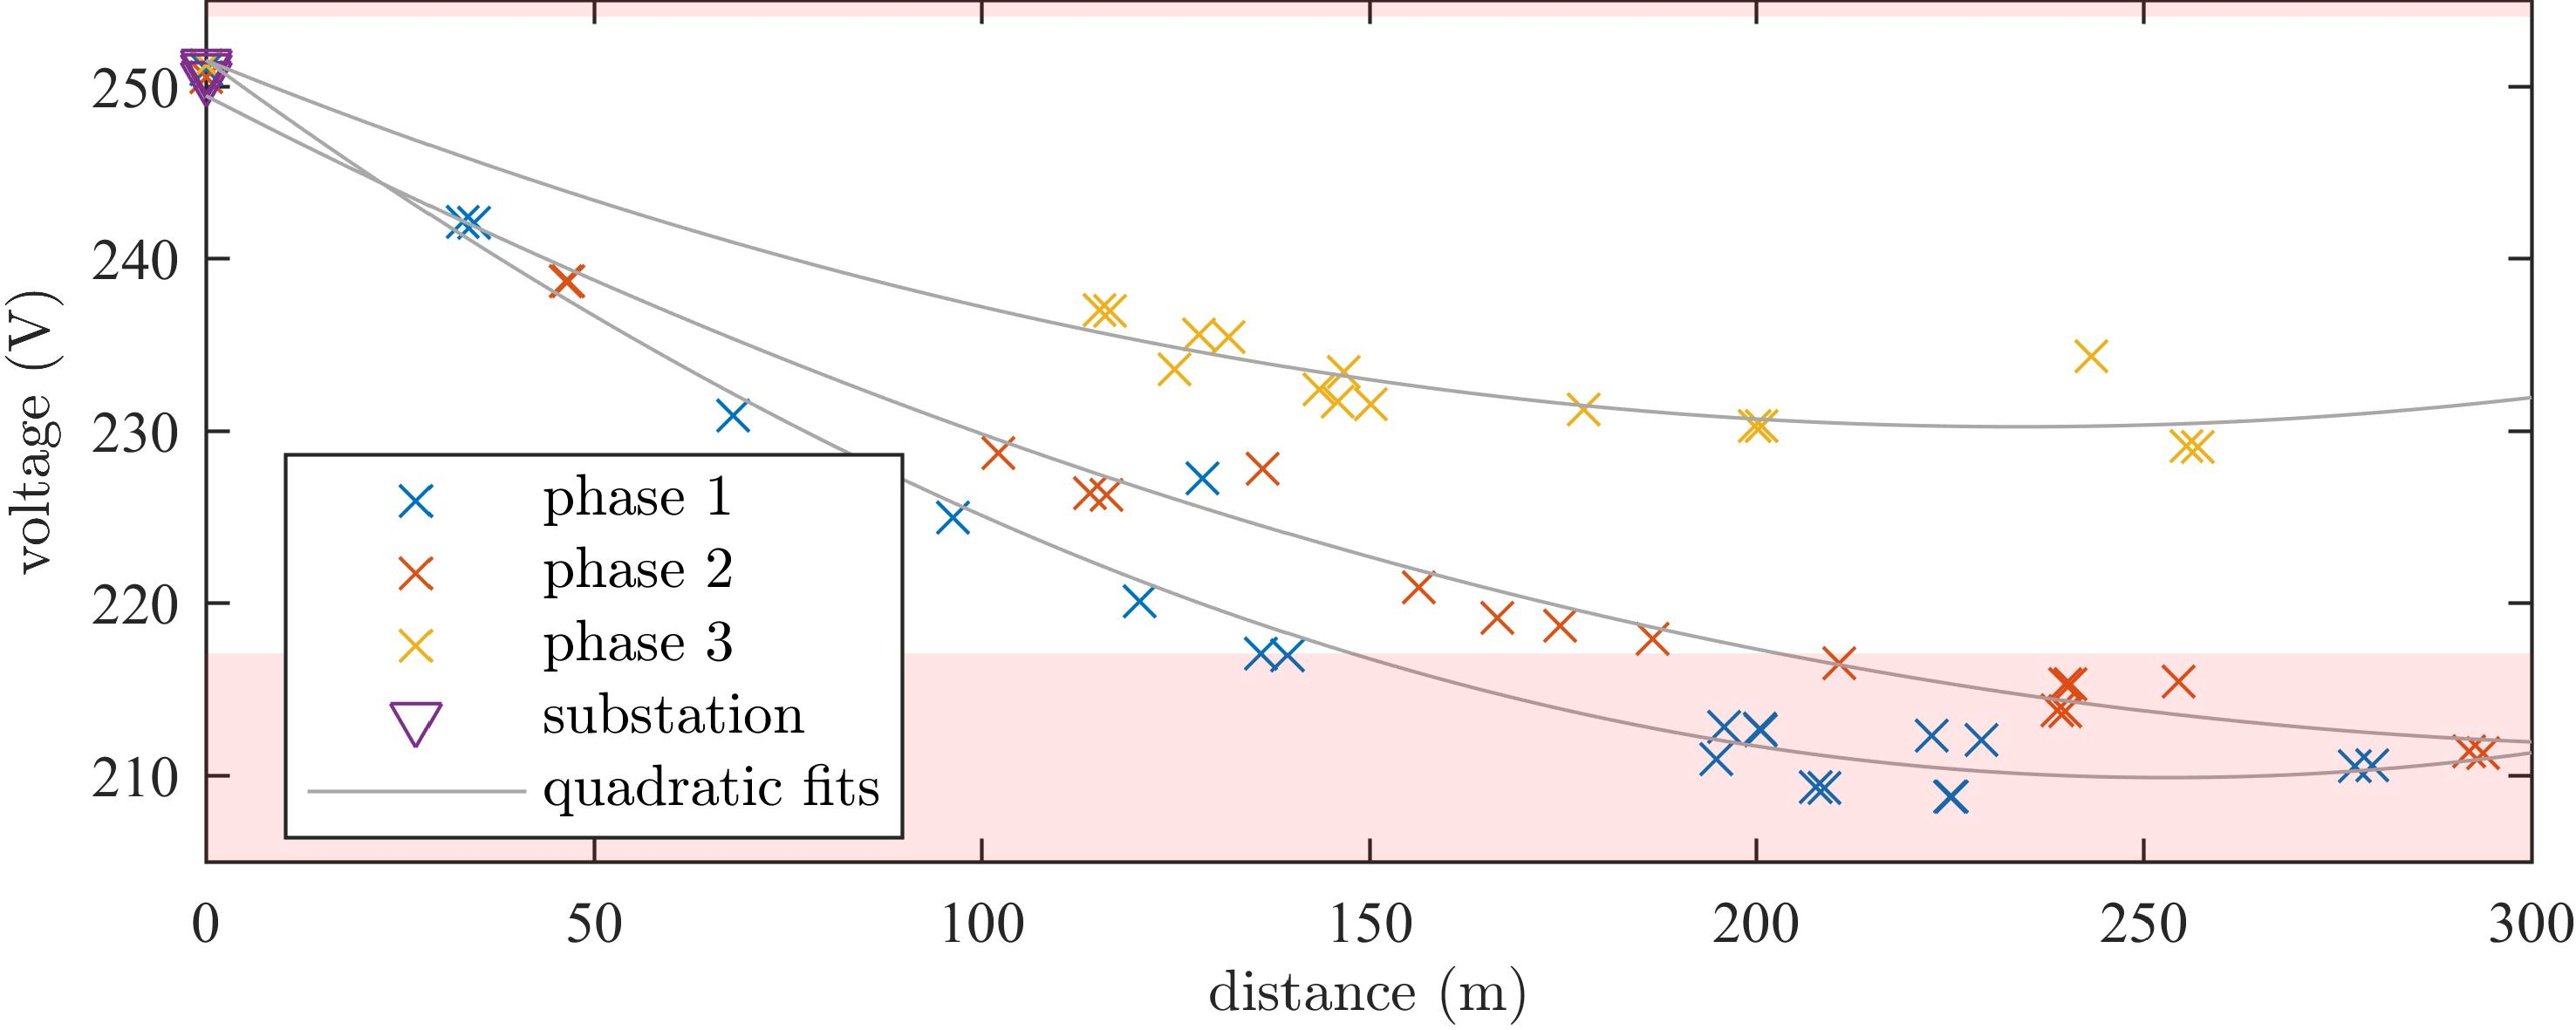
\includegraphics{_chapter1/fig/voltage-drop-for-loads-along-feeder}
	\caption{Voltage at the loads in the IEEE LV Test Case network for a total load of 440kVA against distance between the corresponding load and substation: for the quadratic fit $R^2=58.76\%$}
	\label{ch1:fig:voltage-drop-for-loads-along-feeder}
\end{figure}

\nomenclature[I]{$v_{\text{load},i,\phi}(t)$}{Phase voltage of load $i$ for phase $\phi$ at time $t$, where $\textbf{v}_\text{load}(t) = (v_{\text{load},i,\phi}(t))$ and $v_{\text{load},i,\phi}(t) \in \mathbb{C}$ (Chapter \ref{ch1})}
\nomenclature[I]{$\textbf{v}_\text{load}(t)$}{Multi-phase load voltage vector at time $t$, where $\textbf{v}_\text{load}(t) = (v_{\text{load},i,\phi}(t))$ and $\textbf{v}_\text{load}(t) \in \mathbb{C}^{I\times\Phi}$ (Chapter \ref{ch1})}
\nomenclature[I]{$\zeta_\text{load voltage}(\textbf{v}(t))$}{Voltage deviation cost for load voltage vector $\textbf{v}$ at time $t$ and $\zeta_\text{load voltage}(\textbf{v}(t)) \in \mathbb{R}_{\geq0}$ (Chapter \ref{ch1})}

In this figure, two observations can be made.

\begin{enumerate}
	\item It can be seen that phases are significantly unbalanced. 
	\item Customers further than 200m from the substation are likely to experience low-voltage events.
\end{enumerate}

Although ESMU can reduce the number of such low-voltage events, including a cost for each load would add significant difficulty to the minimisation problem.
Therefore, to solve this problem more efficiently, the previously defined voltage cost function (i.e. Equation \ref{ch1:equ:voltage-deviation}) is expanded to only return a single value from all customer voltages.
More specifically, only the cost deviation is used.
By reducing this number to the worst case, any implemented solver only focuses on the edges of the problem.
This focus is of particular importance, especially if the impact of the ESMU on some customer voltages is comparatively low.
An aggregated voltage deviation cost would potentially obfuscate this impact and prevent the solver from effectively targeting the worst cases.
Therefore, the customer (or load) voltage is defined as $\textbf{v}_\text{load}(t)$, where $\textbf{v}_{load}(t) = (v_{\text{load},i,\phi}(t))$, and used in the new cost function, $\zeta_\text{load voltage}(\textbf{v}_\text{load}(t))$, which is defined as:

\begin{equation}
\begin{split}
	\zeta_\text{load voltage}(\textbf{v}(t)) := \max_{i,\phi}{\zeta_\text{voltage}(v_{i,p}(t))} \\
	\text{ where } i \in \{1, \dots I\} \text{ and } \phi \in \{1, \dots, \Phi\} \text{ and } I \in \mathbb{Z}_{>0} \text{ and } \Phi \in \mathbb{Z}_{>0}
\end{split}
\label{ch1:equ:load-voltage-deviation}
\end{equation}

Here, $i$ represents the customer number out of a total customer count $I$, and $\phi$ represents the phase, out of the phase count $\Phi$, to which the customer is connected.

\subsection{Power related cost functions}
\label{ch1:subsec:powers-related-cost-functions}

Beside meeting voltage constraints, DNOs need to assure that their distribution networks operates both in an efficient and hence ideal manner.
How ideal a three-phase network operates is indicated by its phase unbalance.
This disturbance due to unbalanced phase load may not have an immediate impact, but negative long term effects (e.g. asymmetric load on transformers, rotating machines and increased neutral current) do weaken network assets and cannot be neglected.
The approach by which UK customers are connected to the feeder increases the problem of phase unbalance even more, because the single phase allocation is performed arbitrarily.
Randomly assigning customers' phases was intended to distribute load evenly across all three phases, which in theory should balance the three-phase network load.
In reality however this is not the case.
Even in the unlikely case where the number of customers per phase is the same, the probability that all their loads match is very low.
Therefore, the probability that LV distribution feeders in the UK are unbalanced is very high.

\nomenclature[I]{$\textbf{s}_{ss}(t)$}{Apparent multi-phase power at substation level at time $t$, where $\textbf{s}_{ss}(t) \in \mathbb{C}^\Phi$ (Chapter \ref{ch1})}
\nomenclature[I]{$s_{\text{ss},\phi}(t)$}{Apparent single-phase power at substation level for phase $\phi$ at time $t$, where $\textbf{s}_{ss}(t) = (s_{\text{ss},\phi}(t))$ (Chapter \ref{ch1})}
\nomenclature[I]{$\text{UF}(\textbf{x})$}{Function calculating the Unbalance Factor (UF) for any multidimensional vector $\textbf{x}$, where $\textbf{x} = (x_n)$, $n \in \mathbb{Z}_{>0}$ and $\text{UF}(\textbf{x}) \in \mathbb{R}_{\geq0}$ (Chapter \ref{ch1})}

Substation monitoring is capable of providing reliable three-phase power measurements.
Hence, they can be used as realistic key network parameters to determine the network's phase unbalance.
The American National Standards Institute's (ANSI) definition of Unbalance Factor (UF) is used to calculate the phase unbalance \cite{ANSI-MB-1-2011}:

\begin{equation}
	\text{UF}(\textbf{x}) := \frac{\max_n |\bar{\textbf{x}} - x_n|}{\bar{\textbf{x}}}
	\label{ch1:equ:unbalance-equation}
\end{equation}

Here, $\textbf{x}$ is a three phase vector, where $x_n \in \textbf{x} \text{ for } n=[1, 2, 3]$.
$x_n$ may be a voltage, current or power measurement per phase, but for context of this work $x_n$ was chosen to be the power flow into the network.
For clarity, the notation $\bar{\textbf{s}}$ is used to define the mean of all three phase values.
The mean's definition is give below:

\begin{equation}
	\bar{\textbf{x}} := \frac{1}{3}\sum_n^3{x_i}
\end{equation}

Here, $\textbf{x}$ can be an arbitrary vector, consisting of scalar values $x_n$ (e.g. $x_n$ may be voltage, current or power measurement per phase $n$).
In this context, $x_n$ is chosen to be the power flow into one of the network's phases.
For clarity, the notation of $\overline{\textbf{x}}$ is used to define the mean of the given vector, i.e.:

\begin{equation}
	\overline{\textbf{x}} := \frac{1}{N}\sum_n^N{x_i}
\end{equation}

\nomenclature[I]{$\zeta_\text{unbalance}(\textbf{s}(t))$}{Power unbalance for multi-phase apparent power vector $\textbf{s}$ at time $t$, where $\zeta_\text{unbalance}(\textbf{s}(t)) \in \mathbb{R}_{\geq0}$ (Chapter \ref{ch1})}

Substituting the three-phase substation power vector, $\textbf{s}_{ss}(t)$ (where $\textbf{s}_{ss} = (s_{\text{ss},\phi})$), for $\textbf{x}$, allows the formulation of another cost, i.e. the ``unbalance'' cost, $\zeta_\text{unbalance}(\textbf{s}_{ss}(t))$, which is defined as:

\begin{equation}
	\begin{split}
		\zeta_\text{unbalance}(\textbf{s}(t)):=&\text{UF}(\textbf{s}(t)) - 1 \forall t\\
		=&\frac{\max_p\left|\overline{\textbf{s}(t)} - s_{p}(t)\right|}{\overline{\textbf{s}(t)}} \forall t\\
		=&\frac{\max_p\left|\left(\frac{1}{P}\sum_p^P{s_{p}(t)}\right) - s_{p}(t)\right|}{\frac{1}{P}\sum_p^P{s_{p}(t)}} \forall t\\
		&\text{where } p \in [1, 2, \dots P]
	\end{split}
	\label{ch1:equ:unbalance-cost}
\end{equation}


Since the lowest value of $\text{UF}(\textbf{x})$ is one, the corresponding cost function had to be adjusted in order to reach a minimum value of zero instead.
A sample illustration, showing how this cost behaves as phase unbalance increases, is included in the Figure \ref{ch1:fig:power-unbalance}.

\begin{figure}\centering
	
\includegraphics[width=5cm]{foo}
	\caption{Sample network imbalance for different phase loadings as defined in ANSI/NEMA MG 1-2011}
	\label{ch1:fig:power-unbalance}
\end{figure}

\nomenclature[I]{$\zeta_\text{PF}(\textbf{s}(t))$}{Power Factor (PF) cost function for multi-phase apparent power vector $\textbf{s}$ at time $t$, where $\zeta_\text{PF}(\textbf{s}(t)) \in \mathbb{R}_{\geq0}$ (Chapter \ref{ch1})}

Here, it can be seen how $\zeta_\text{unbalance}(\textbf{s}(t))$ rises with an increasing separation of the three-phase power values.
Additionally, to assess the effective utilisation of the power distribution network, deviation from a unity Power Factor (PF) is also formulated as a cost.
PF is the ratio between active (p) and apparent power (s), and gives an indication of how much ``good'' power is being consumed by the system\footnote{Reactive power is used to maintain magnetic fields in rotating machines, yet this can be supplied by local reactive power compensators and thus need not occupy otherwise free power transmission resources.}.
Experts would agree that keeping PF of a system close to unity indicates that it only requires active power to operate, which implies that uses the lowest possible amount of power transmission resources.
In order to indicate the proximity to unity PF, a corresponding cost, $\zeta_\text{PF}(\textbf{s}_{ss}(t))$, us used, which is defined as:

\begin{equation}
	\zeta_\text{PF}(\textbf{s}(t)):= \sum_{\phi=1}^{\Phi}\frac{\text{Re}(s_\phi(t))}{|s_\phi(t)|} - 1 \forall t \text{ where } s_\phi(t) \in \textbf{s}(t) \text{ and } \Phi \in \mathbb{Z}^{>0}
\label{ch1:equ:power-factor}
\end{equation}

\nomenclature[I]{$\zeta_\text{neutral load}(\textbf{s}(t))$}{Neutral load cost function for multi-phase apparent power vector $\textbf{s}$ at time $t$, where $\zeta_\text{neutral load}(\textbf{s}(t)) \in \mathbb{R}_{\geq0}$ (Chapter \ref{ch1})}

Any deviation from a unity PF per phase increases the associated cost, whilst achieving a perfect PF for each phase results in a total cost of zero.
In perfectly balanced systems that operate at unity PF, all three phases are $120^\circ$ out of phase, and the sum of their instantaneous powers should equate to zero.
This zero-sum also indicates, that no neutral current is flowing in the system.
However, in an unbalanced system that operates at non-unity PF, the power transmitted through the neutral conductor can significantly deviate from zero.
The negative impact of transmitting power through the neutral conductor is further amplified, since typical power distribution cables often use neutral conductors with significantly smaller cross-section areas than those used as line conductors.
Results of any such additional power flow in the neutral conductor are further deviation of neutral voltages from ground, increased losses, and quicker exhaustion of the neutral conductor's power carrying capability (making the system become more prone to failures).
To address this last point, a ``neutral load'' cost, $\zeta_\text{neutral load}(\textbf{s}_{ss}(t))$, is defined:

\begin{equation}
	\zeta_\text{neutral load}(\textbf{s}(t)) := \left|\sum_{\phi=1}^{\Phi} s_\phi(t)e^{\frac{j2\pi\phi}{\Phi}}\right| \text{ where } \textbf{s}(t) = (s_\phi(t)) \text{ and } \Phi \in \mathbb{Z}_{>0}
\label{ch1:equ:neutral-load}
\end{equation}

In this cost function, for a three-phase scenario, each single-phase power, $s_{\text{ss},\phi}(t)$, is therefore rotated by an integer multiple of $120^\circ$ in the complex plane, before adding them in order to obtain the neutral load vector.
It is the magnitude of this apparent power vector is computed, which is then used as the resultant cost.
Power losses have already been mentioned.
In comparison to the losses of the entire electricity grid, losses in a LV distribution network are negligibly small.
Nonetheless, the aggregate effect of reducing those losses could have a noticeable impact on both network efficiency and maximising profit margins (after all, nobody pays for undelivered energy).
For example, in the high load scenario that was simulated in in Section \ref{ch1:subsec:voltages-related-cost-functions}, distribution losses were calculated as 58kW.
This equates to 12\% of the total network power, however, losses would be noticeably lower during normal network operation, e.g. a maximum of 5\%.
The rising proportion of losses, as uniform network load is continuously increased, is shown in Figure \ref{ch1:fig:losses-against-network-demand}.

\begin{figure}\centering
	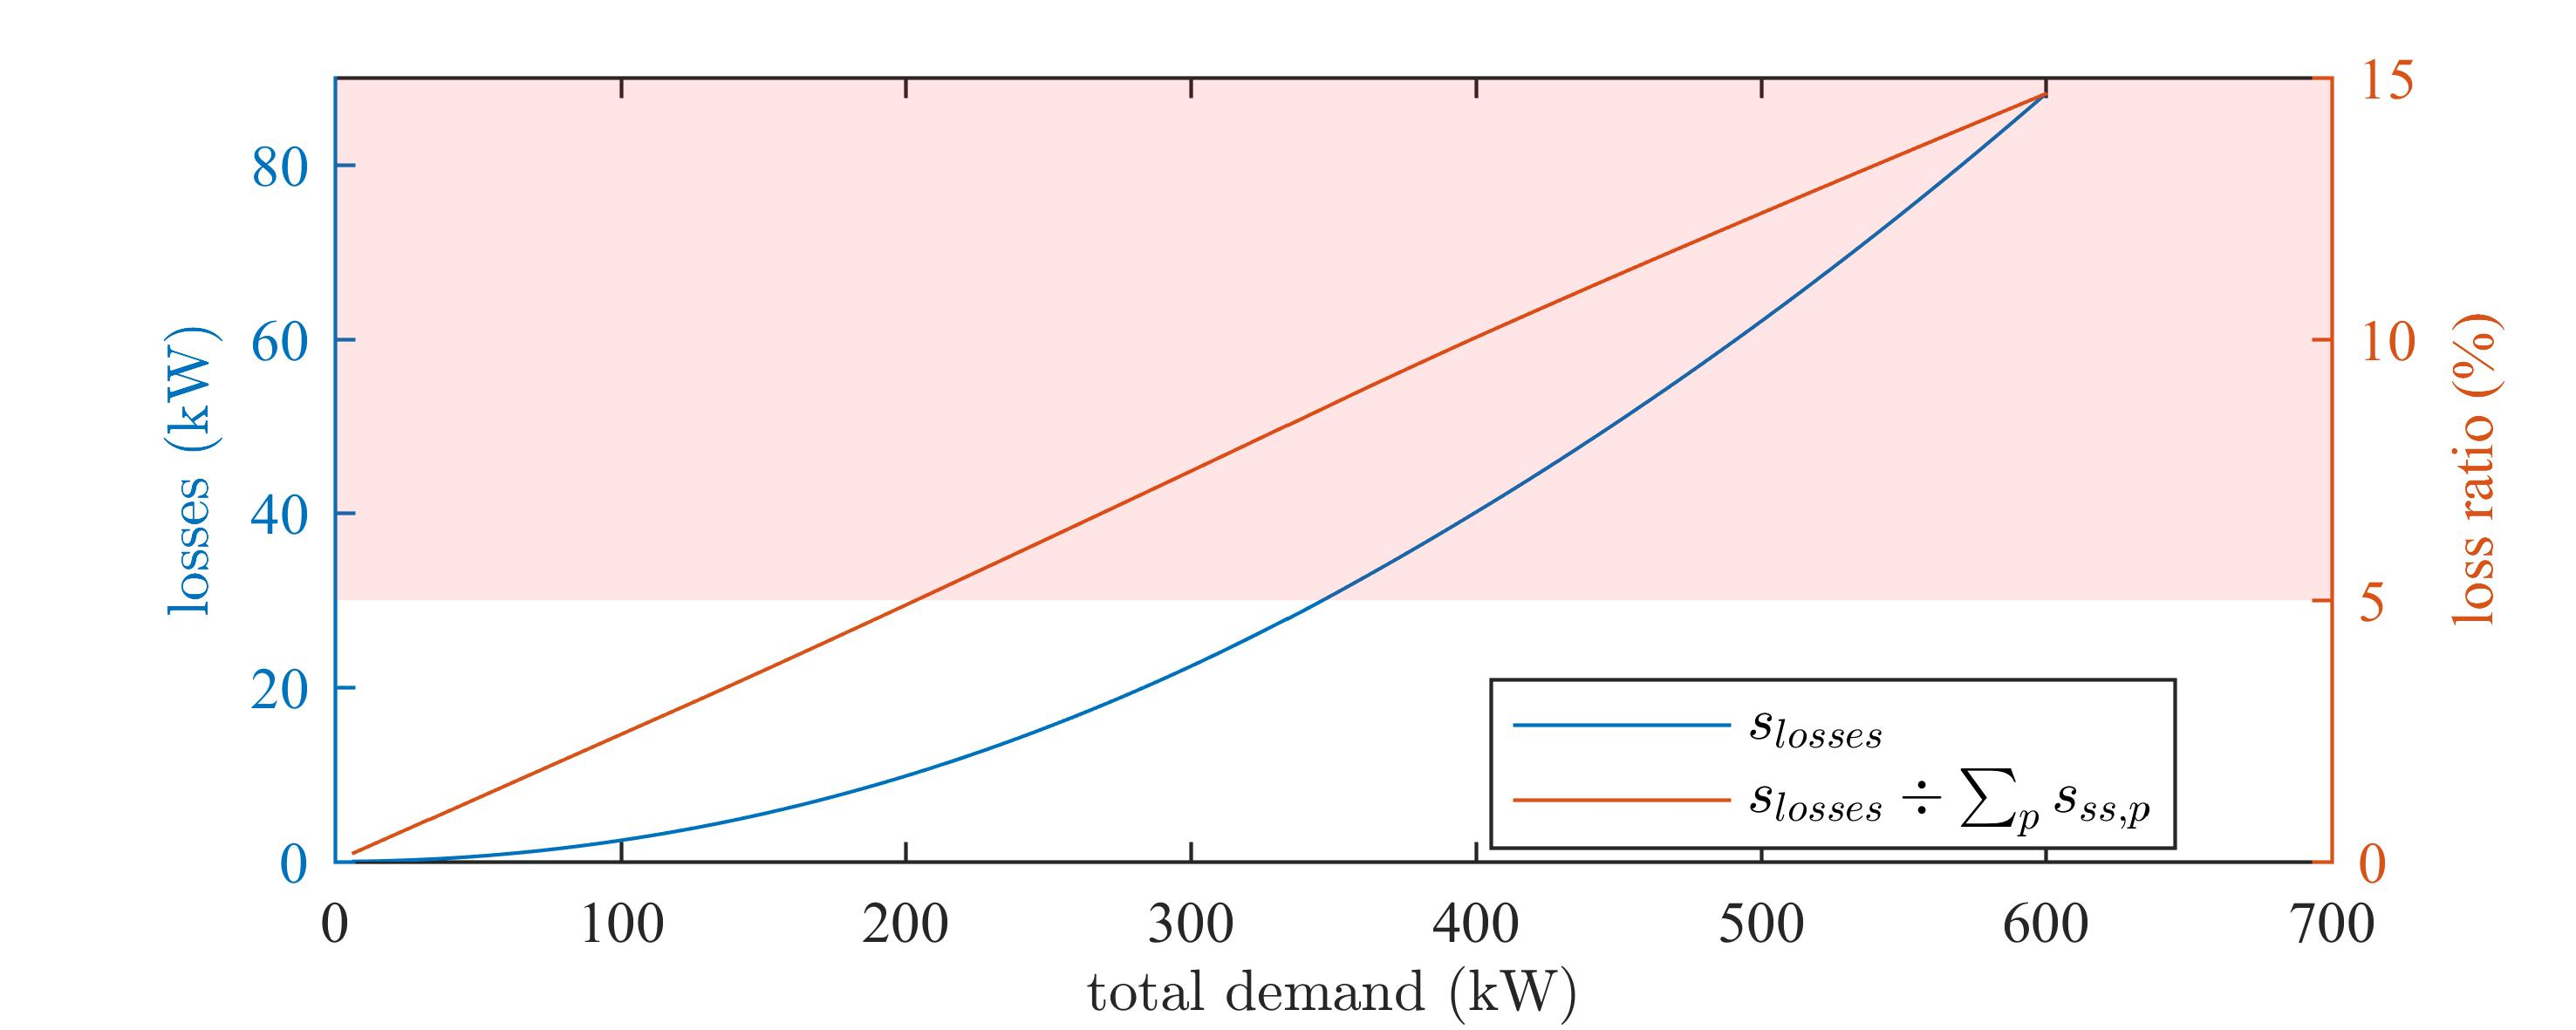
\includegraphics{_chapter1/fig/losses-against-network-demand}
	\caption{Losses against increasing power demand}
	\label{ch1:fig:losses-against-network-demand}
\end{figure}

\nomenclature[I]{$\zeta_\text{losses}(s(t))$}{Losses based cost function, where $\zeta_\text{losses}(s(t)) \in \mathbb{R}_{\geq0}$ (Chapter \ref{ch1})}
\nomenclature[I]{$s_\text{losses}(t)$}{Total apparent power losses in the network $s_\text{losses}(t) \in \mathbb{C}$ (Chapter \ref{ch1})}

In Figure \ref{ch1:fig:losses-against-network-demand}, the region where losses exceed 5\% of the total network power is highlighted in red.
Whilst these losses are easily obtained from power flow simulations, in reality, distribution losses cannot be determined with such ease.
Therefore, the network losses, $s_\text{losses}(t)$, are seen as theoretical key network parameters and they are used in the final power related cost, $\zeta_\text{losses}(s(t))$, which is defined as folllows:

\begin{equation}
	\zeta_\text{losses}(s(t)) := |s(t)| 
	\label{ch1:equ:losses}
\end{equation}

\subsection{Current related cost functions}
\label{ch1:subsec:currents-related-cost-functions}

\nomenclature[I]{$I_\text{fuse}$}{Nominal fuse rating at substation, where $I_\text{fuse} \in \mathbb{R}$ (Chapter \ref{ch1})}
\nomenclature[I]{$i_{\text{ss},\phi}(t)$}{Single-phase substation current for phase $\phi$ at time $t$, where $i_{\text{ss},\phi}(t) \in \mathbb{R}$ (Chapter \ref{ch1})}
\nomenclature[I]{$\textbf{i}_{ss}(t)$}{Multi-phase substation current at time $t$, where $\textbf{i}_{ss}(t) \in \mathbb{R}^\Phi$ (Chapter \ref{ch1})}
\nomenclature[I]{$\zeta_\text{fuse utilisation}(\textbf{i}_{ss}(t))$}{Fuse utilisation cost, derived from multi-phase substation current vector $\textbf{i}_{ss}$ at time $t$, where $\zeta_\text{fuse utilisation}(\textbf{i}_{ss}(t)) \in \mathbb{R}_{\geq0}$ (Chapter \ref{ch1})}

Having addressed voltage deviation and inefficient network operation, physical network limits have not yet been taken into account: i.e. the current carrying capabilities of the cables.
Heat, i.e. losses that are caused by the line's impedance, deteriorates the cable over time.
Therefore, cables have an assigned thermal rating which should not be exceeded in order to minimise permanent cable damage and mitigate possible network failure.
At substation level, to prevent over-currents, fuses or reclosers are installed that will disconnect the network under fault or high current conditions.
To quantify whether the substation fuse is approaching its tripping point, its nominal fuse rating, $I_\text{fuse}$, is used.
For the context of this work, $I_\text{fuse}$, is a static value which must not be exceeded.
Using the three-phase current vector, $\textbf{i}_{ss}(t)$ (obtained via substation monitoring, where $\textbf{i}_{ss}(t) = (i_{\text{ss},\phi}(t))$) a cost, $\zeta_\text{fuse utilisation}(\textbf{i}_{ss}(t))$, is formulated, and defined as follows:

\begin{equation}
	\zeta_\text{fuse utilisation}(\textbf{i}(t)) :=%
	\left|\frac{\sum_{\phi=1}^{\Phi}{i_\phi(t)}}{I_\text{fuse}}\right|^2%
	\text{ where } \phi \in \{1, \dots, \Phi\}%
	\text{ and } \Phi \in \mathbb{Z}_{>0}
	\label{ch1:equ:fuse-utilisation}
\end{equation}

In the Figure \ref{ch1:fig:fuse-utilisation}, a plot has been included to illustrate how this quadratic cost behaves as substation current increases.
For this simple case, the substation line rating was set as $i_{fuse}=400\text{A}$, and the total substation current is the sum of all three phase currents.
The red area indicates the region where current exceeds the fuse's nominal rating.

\begin{figure}
	
\includegraphics[width=5cm]{foo}
	\caption{Cost of line or fuse utilisation against network current}
	\label{ch1:fig:fuse-utilisation}
\end{figure}

\nomenclature[I]{$l$}{Line number, where $l \in [1, \dots, L]$ (Chapter \ref{ch1})}
\nomenclature[I]{$L$}{Number of lines, where $L \in \mathbb{Z}_{>0}$ (Chapter \ref{ch1})}
\nomenclature[I]{$i_{\text{line},l,\phi}(t)$}{Single-phase line current for phase $\phi$ of line $l$ at time $t$, where $i_{\text{line},l,\phi}(t) \in \mathbb{R}$ (Chapter \ref{ch1})}
\nomenclature[I]{$\textbf{i}_\text{line}(t)$}{Multi-phase line currents at time $t$, where $\textbf{i}_\text{line}(t) = (i_{\text{line},l,\phi}(t))$, and $\textbf{i}_\text{line}(t) \in \mathbb{R}^{L\times\Phi}$ (Chapter \ref{ch1})}
\nomenclature[I]{$I_{\text{nom},l}$}{Nominal line current for line $l$, $I_{\text{nom},l} \in \mathbb{R}$ (Chapter \ref{ch1})}

In addition to the currents flowing through the substation's fuse, currents flowing through all lines in the network may also be considered.
Just like voltage levels at each customer, line currents are also seen as theoretical key network parameters, since they cannot easily be obtained.
Generally, as the distance to the substation increases fewer ``down stream'' customers are connected to a radially expanding feeder, and therefore cables can be scaled down, i.e. to save cost.
However with the expected uptake of LCTs, feeders are expected to deliver increasingly larger currents throughout all lines.
For smaller lines at the network edge, these currents may increase to a magnitude larger than their nominal ratings.
Therefore, the fuse current cost is expanded to take into account all line currents, $i_{\text{line},l,\phi}(t)$, and their nominal ratings, $I_{\text{nom}, l}$.
Here $l$ represents the line number and $\phi$ the phase of that line.
Collecting them in $\textbf{i}_{line}(t)$ (where $\textbf{i}_\text{line}(t) = (i_{\text{line},l,\phi}(t))$) allows the formulation of an extended line utilisation cost, $\zeta_\text{line utilisation}(\textbf{i}_\text{line}(t))$, which is defined as follows:

\begin{equation}
\begin{split}
	\zeta_\text{line utilisation}(\textbf{i}(t)) :=
	\max_{l}{\left(\frac{\sum_{\phi=1}^{P}{i_{l,\phi}(t)}}{I_{\text{nom},l}}\right)^2} \\
	\text{where } l \in \{1, \dots, L\} \text{ and } \phi \in \{1, \dots, \Phi\} \text{ and } L \in \mathbb{Z}_{>0} \text{ and } \Phi \in \mathbb{Z}_{>0}
\end{split}
\label{ch1:equ:line-utilisation}
\end{equation}

Similar to Equation \ref{ch1:equ:load-voltage-deviation}, this cost function only considers the maximum line utilisation in order to reduce computational burden without decreasing any parameter sensitivity.
